\chapter{Introduction}
\label{chapter:body}
\thispagestyle{myheadings}
\setcounter{tocdepth}{1}
% set this to the location of the figures for this chapter. it may
% also want to be ../Figures/2_Body/ or something. make sure that
% it has a trailing directory separator (i.e., '/')!
\graphicspath{{1_Intro/Figures/}}

Incoherent scatter radar (ISR), like all scientific instruments, is a testament to humankind's desire to understand the world around it. This even more so because they are generally very large and complicated systems that use substantial amounts of power, in the range of megawatts.
Incoherent scatter radar (ISR) has been in use since the 1950s\cite{gordon58}. These systems work by monitoring the reflected electromagnetic radiation from free electrons in the ionosphere. This scatter has a specific spectral distribution from which various parameters can be determined. Unlike other ground based measures this system can give direct measurements of various plasma parameters including electron density ($N_e$), electron temperature ($T_e$), ion temperature ($T_i$) and ion velocity ($V_i$). 

Until recently these systems were constructed using single, mechanically steered antennas. Because of this the rate that the look angle can change is limited by the mechanical speed of the \jcom{doesn't sound right}{antenna pointing mechanism.} The newest generation of ISR systems are now taking advantage of electronically scanning phased array (ESPA), which allow for a near instantaneous change in the radar look direction. This technological development gives researchers new flexibility in designing experiments and can even create a three dimensional view of the plasma parameters in the ionosphere. 

Examples of these new systems include The Advance Modular Incoherent Scatter Radars (AMISR), that have been developed and placed in Poker Flat Alaska and in Resolute Bay Canada. These systems have already started to give unprecedented views in the ionosphere and upper atmosphere. Currently EISCAT-3D is being developed as well and is expect do give even greater views due to the multi-static set up.

\section{Purpose}

For this dissertation we will be proposing to improve the spatial and time sampling of the ISR systems.  New phase array radar systems have allowed for an unprecedented amount of flexibility in sampling the environment.  As such there has been no optimal way developed as of yet to sample this space.  Currently ISR systems integrate their spectral estimate in time only.  In order to get a statistical desirability of their measurements these systems may have to integrate for a long period of time.  It may be possible to integrate across different beams if stationarity can be found.  Other techniques could also be investigated such as well to try to improve the ISR measurements.


\section{Ionosphere and Phenomena}
The ionosphere is the area of partially ionized gas, or plasma, surrounding the earth and in a way is like an interface between the earth and outer space\cite{kellybook}. In order to understand the behavior of the plasma in the ionosphere one needs to use electromagnetics governed by Maxwells Equations seen in Equations \ref{eqn:max1} and \ref{eqn:max2},

\begin{eqnarray}
\label{eqn:max1}
\nabla \cdot \vec{E} = \frac{\rho}{\epsilon_0}\  &&\nabla  \cdot \vec{B} = 0 \nonumber \\
\nabla  \times \vec{E} = - \frac{\partial B}{\partial t} && \nabla  \times \vec{B} = \mu_{0}\vec{J} +
\mu_{0}\epsilon_{0}\frac{\partial E}{\partial t}
\end{eqnarray}

\begin{equation}
\label{eqn:max2}
\frac{\partial \rho}{\partial t}+\nabla \cdot \vec{J} = 0
\end{equation}
 
\noindent where $\vec{E}$ is the electric field, $\vec{B}$ is the magnetic field, $\vec{J}$ is the current density, $\mu_0$ is the vacuum permeability and $\epsilon_0$ is the vacuum permittivity.

The high latitude ionosphere is of special interest due to the number of different phenomena that occur in this region.  These phenomena include but are not limited to aurora borealis, polar cap plasma patches and particle precipitation events.  

The following is a listing of examples various types of high latitude ionosphere events grouped by specific behavior that is of interest the ISR sampling problem.

\begin{figure}[!t]
\centering
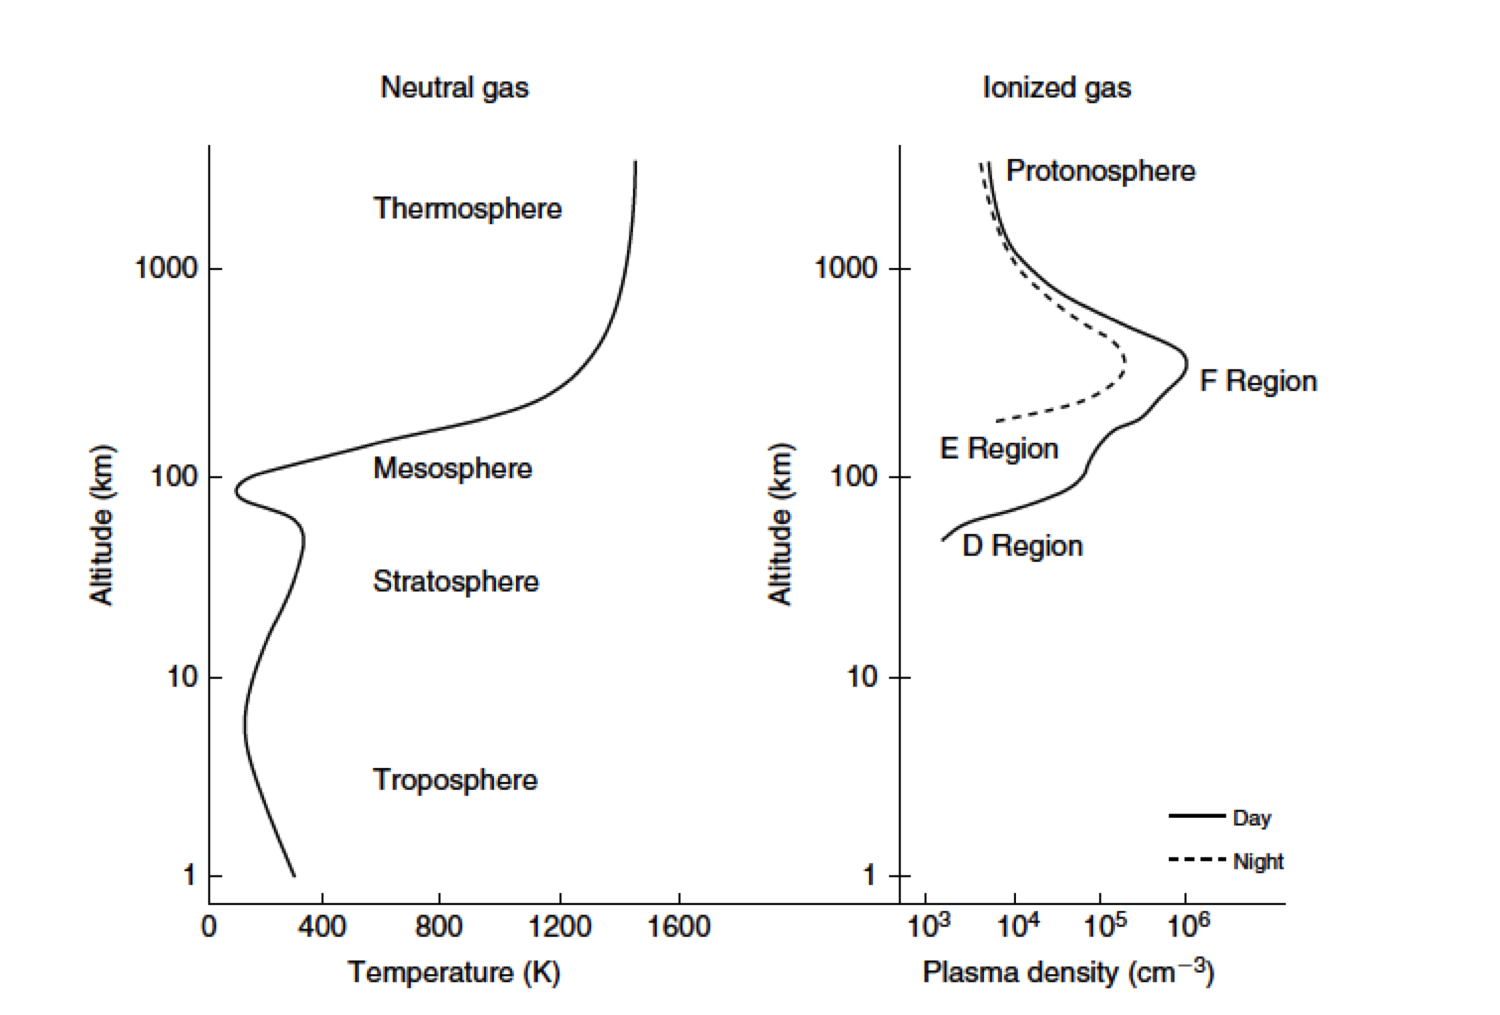
\includegraphics[width=5in]{altvsparams}
% where an .eps filename suffix will be assumed under latex, 
% and a .pdf suffix will be assumed for pdflatex; or what has been declared
% via \DeclareGraphicsExtensions.
\caption{Example profiles of neutral temperature and plasma density from \cite{kellybook}}
\label{fig:singlefilt}
\end{figure}
%These systems right now are all located in what can be considered the high latitude ionosphere.  This is a highly dynamic environment in both time and space.  The plasma can change very quickly due to the physics of the environment.  These types of events can be classified into a number of types that will be of interest to this type of sampling problem.

\subsection*{High Spatial Gradient Events}
Polar cap patches are examples where of high spatial gradients in various plasma parameters \cite{Dahlgren:2012dq},\cite{dahlgren2012di}.  In the polar cap large blobs of plasma with elevated electron density travel from the dayside to the night side ionosphere.  These patches can play a large role in plasma transport within the polar ionosphere and interfere with radio transmission as well.  Examples of sensor data that show these patches can be seen in Figure \ref{fig:patches}.

\begin{figure}[!t]
\centering
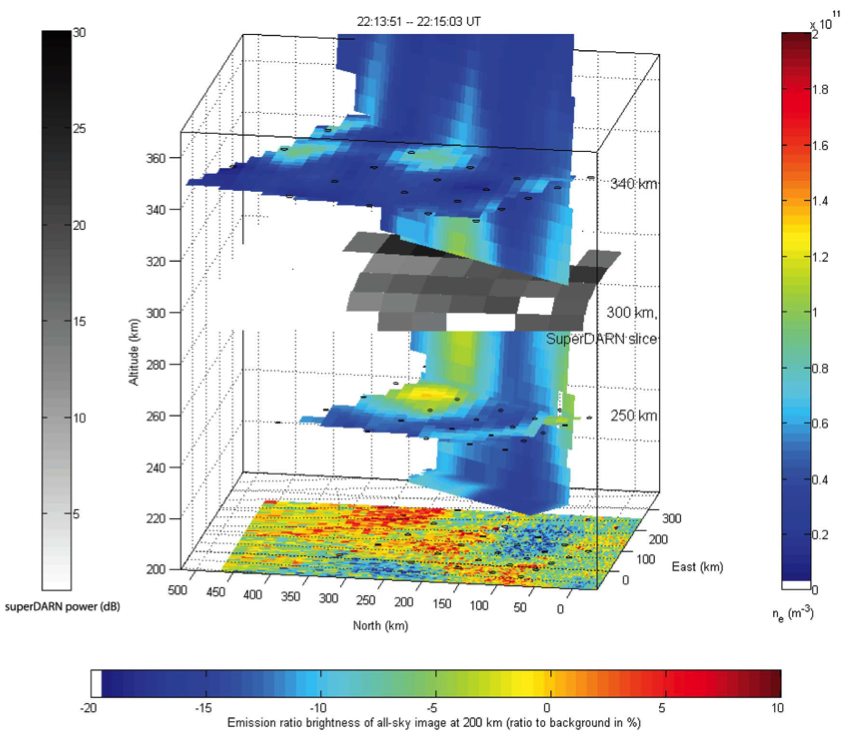
\includegraphics[width=4.0in]{patches}
% where an .eps filename suffix will be assumed under latex, 
% and a .pdf suffix will be assumed for pdflatex; or what has been declared
% via \DeclareGraphicsExtensions.
\caption{Example of polar cap patches seen in RISR and SuperDARN, from \cite{Dahlgren:2012dq}}
\label{fig:patches}
\end{figure}

Large horizontal gradients also occur during geomagnetic storms which can produce large flows.  This can create large disparities in Ion temperature as heating is occurring \cite{Zettergren:2008ba},\cite{semeter:plasmatransport2012}.  During these storms ion temperatures can go from 500$^\circ$ K to over 1500$^\circ$ K in the order of kilometers.

These high gradient events can cause some upridictible errors where two plasma population interface.  These errors can be quite complex due to the nonlinear nature of the inversion process\cite{Vallinkoski1990665}.  Similar behavior has been observed during times of auroral turbulence where shear flows seems to have caused non isotropic temperature measurements\cite{knudsen1993}. 
%\subsection*{Small Structure Events}
%\cite{semeter2010CI}
\subsection*{High Speed Events}
At times the ionosphere can be come locally unstable this can create a number of different types of turbulent events. Langmuir turbulence can create coherent structures that will be detected by ISR systems \cite{akbari:2013lt}.  These structures change on the order of one pulse repetition interval of the radar.

%Resolving these high speed events are of great interest but also a challenge.  In ISR systems each pulse is used as a sample of a spectral averaging procedure.  It is assumed that these spectrums are identical independent samples.  If spectrum changes during this time, errors in the measurement could take place.  These errors are often unpredictable due to the nonlinear fitting used to fit the spectrum with the plasma parameters.
 %\cite{Dahlgren:2013ip}
%In the past researchers have studied errors associated with different plasma distributions mixing together.  These errors can be quite complex due to the nonlinear nature of the inversion process\cite{Vallinkoski1990665}.  Similar behavior has been observed during times of auroral turbulence where shear flows seems to have caused non isotropic temperature measurements\cite{knudsen1993}. 
\section{Radar Sampling}


The main way to look at Doppler in hard-target radar is to assume it is a multiplication of the radar signal $s(t)$ with a simple single complex exponential

\begin{equation}
\label{simpledop}
s_d(t) = s(t)e^{j\omega_d t},
\end{equation}
 
\noindent where $\omega_d$ is the Doppler frequency of the target or object.  If we say have multiple targets each with their own Doppler frequency and their own weighting, which would represent a relative scattering to each components,  we can represent that signal as the following

\begin{equation}
\label{multiDop}
\displaystyle s_d(t) = \sum_{n}^{N} s(t)X(\omega_n)e^{j\omega_{n} t}.
\end{equation}

\noindent Extending this to a continuum of signals each at each Doppler frequency this becomes

\begin{equation}
\label{conDop}
s_d(t) = \int s(t) X(\omega)e^{j\omega t}.
\end{equation}
\noindent Pulling the $s(t)$ term out of the integral we can see that we are taking the Fourier transform of this relative weighting between each of the scatters and then multiplying it with the signal.  Using simple Fourier properties we can see that this equivalent to a convolution in frequency space of the spectrum of the original radar signal and the Doppler spectrum with the collection of targets.  

The final form of the signal spectrum with Doppler added can be shown as the following

\begin{equation}
\label{finalDop}
s_d(t) = \int \left[\int S(\lambda)X(\lambda-\omega)d\lambda\right] e^{j\omega t}d\omega.
\end{equation}

\noindent This shows that the measured Doppler on the radar signal can be formulated as the convolution of the Fourier transform of radar's signal along with the Doppler spectrum of the target.

\section*{Applying the Model To Pulse Doppler Radar}

In pulse-Doppler (PD) radar a succession of pulses are sent out modulated by the carrier frequency $f_c$.  Each pulse scatters off of the target and which imparts a Doppler frequency $\omega_d = 2\pi f_c \frac{2v}{c}$, where $v$ is the target velocity and $c$ is the speed of light.  This representation of the Doppler frequency is only valid if the target is non-relativistic.  In the case where we are looking at a single target the return of the $m^{th}$ pulse can be represented in the following way\cite{richards:fundamentalsigproc}

\begin{equation}
\label{pdpulse}
y(t) =  A(t)e^{j\phi}e^{j\omega_dmT},
\end{equation}

\noindent where $T$ is the pulse repetition interval (PRI).  In this case each pulse is sampling the Doppler spectrum at a rate of the pulse repetition frequency (PRF).  Using traditional PD processing the PRF determines the maximum unambiguous Doppler frequency.  For example if one wants a system with a carrier frequency of 10 GHz that will resolve a target going the speed of sound with aliasing in Doppler (approximately 340 m/s) that system must have a PRF greater than 45 kHz if one uses the Nyquist theorem.   

To get the final measurement of this spectrum often a Discrete Fourier transform is applied.  When the data arrives to the radar it is sampled in to specific range gates and pulse samples.  Pulse compression is applied across range to help to localize the signal in range.  This operation is basically applying a filter that is the time reversed conjugate of the base band pulse.  After pulse compression operation Discrete Fourier Transforms are taken across the pulse dimension in each range bin.   The final result is commonly referred to as a range-Doppler map.


%%%%%%%%%%%%%%%%%%%%%%%%%%%%%%%%%%%%%%%%%%%%%%%%%%
\subsection{Applying the model to ISR}
In some radar modalities the system is attempting to measure numerous targets.  The number of targets grows the scatters resemble more of a distribution than a single scatterer.  In the case of ISR the radar is trying to sample the velocity spectrum of the distribution of electrons in the upper atmosphere and ionosphere.  

In ISR the goal of the system is often to sample what is called the ion-line spectrum.  From Dougherty and Farley's 1960 paper \cite{dougherty:farley1960} the normalized spectrum can be formulated as 

\begin{equation}
\label{ionline}
X(\theta) = \frac{e^{-\theta^2}}{\pi \theta^2 e^{-2\theta^2}+(2-I(\theta))^2},
\end{equation}

\noindent where $\theta=(\omega/k)\sqrt{m_i/(2KT_i)}$, $K$ is Boltzman's Constant and $I(\theta)$ can be represented as the following:
\begin{equation}
\label{Ifunc}
I(\theta) = 2\theta e^{-\theta^2}\int_0^\theta e^{t^2}dt.
\end{equation}

% make ISR spectra


One can see in this formulation that the distribution is actually dependent on the thermal velocity of the ions $\sqrt{2KT_i/m_i}$.  If one multiplies this velocity by the wavenumber $k$ of the radar we actually get a Doppler frequency.  This term is basically a normalization of the frequency space of the distribution to what would be the Doppler of the average thermal speed.  The distribution $X(\theta)$ is basically the distribution of the scatterers at these different speeds.

To sample this spectrum one needs a process that can sample this frequency response.  Although the function in Equation \ref{ionline} has a number of assumptions built in one could still use it as a way to get a feel for what type of sampling frequencies are required.  If we look at Figure \ref{ionlinefig} we can see it seems to have no appreciable content beyond $3\omega_\theta$, thus one needs a sensor that can sample at a frequency of at least $6\omega_\theta$ if we are using the Nyquist theorem.  To give a rough example we can say that one wants to look at hydrogen ions at a  temperature 600 Kelvin with a sensor that has a center frequency of 450 MHz \footnotemark[1].  This will yield an $\omega_\theta/2\pi$ of about 2 kHz and in order to sample that spectrum one would need to sample at about 12 kHz just to get this spectrum.
  
\footnotetext[1]{This is a very simple example and probably not best for the ionosphere.  I probably should use Oxygen ions or some other species for this example.}

If one were to use a pulse-Doppler sort of approach to sampling the process used in the previous example one would need a PRF of about 12KHz.  This PRF would only allow the pulse scatter off of a targets that are no more farther then 125km out.  This would not work for ionosphere measurement when one want to measure out 700km. 

In order to measure this spectrum ISR systems often use an intra-pulse autocorrelation method to measure the Ion-line spectrum.  To do this a pulse with a long time width is sent.  The length is often on the order of a number of range bins.  It is assumed that the plasma from different range's is uncorrelated but since the pulse is longer than a range bin energy scattered from other ranges are summed into other range bins.  Once the correlations are formed a Fourier transform is taken of the autocorrelation functions (ACF), thus yielding a power spectrum for each range.  This operation can also be described in terms of a Wigner-Ville distribution in that we are taking the Fourier transform of a time dependent correlation.\footnotemark[2] This spectrum is again the Doppler spectrum of the distribution of targets though and one is left with a range-Doppler map.

In a sense pulse-Doppler and ISR are attempting to measure the same quality, a Doppler spectrum of some target but they just have different measurement methods.  In PD radar the Doppler spectrum is measured across the pulses while in ISR the Doppler spectrum is measured within the pulse itself.  

This is mainly because of what the different systems are trying to measure.  In most PD systems the required sample rate of the Doppler does not cause high enough PRFs to cause range ambiguities.  Also in detection systems where point targets are being detected range (and Doppler) ambiguities can often be corrected.

In ISR the target being observed is a distribution of scatterers with a fairly large Doppler bandwidth.  The large Doppler bandwidth along with the need to measure parameters at far ranges requires one to develop the Doppler spectrum using information that is available within a pulse.  The pulses themselves are basically used as samples in an averaging of the autocorrelation function to develop a statistically significant representation of the spectrum.
\footnotetext[2]{ I need to work on the wording of this paragraph and add examples}


\section{Contributions}
Specific contributions of this research are summarized below.

\begin{enumerate}
\item Development of a theoretical framework for the forward model of 3-D ISR plasma parameter reconstructions.
\item Creating a framework full simulation of an ISR system that can which yield synthetic complex voltages.
\item A software package, named STISRS(Space-Time ISR Simulator), has be derived from this framework has been made available to other researchers.
\item A detailed analysis of the simulation framework using STISRS.
\item A new method for inverting the forward model 3-D ISR plasma parameter reconstructions.
\end{enumerate}